\documentclass{article} % Defines the document class, article is commonly used
\usepackage[shortlabels]{enumitem}
\usepackage{amsmath}    % Allows for more advanced math formatting
\usepackage{amssymb}    % Provides additional mathematical symbols
\usepackage{amsthm}     % \qed
\usepackage{graphicx}   % image
\usepackage{float}      % image placement
\usepackage{hyperref}
\hypersetup{
    colorlinks=true,       % false: boxed links; true: colored links
    linkcolor=black,       % color of internal links
}
\usepackage[margin=1.5in]{geometry}
\usepackage{siunitx}

\begin{document}

\title{EEC133 HW3}
\author{Tao Wang}
\date{\today}

\maketitle
\tableofcontents

\section{A few simple dipole antennas}
\begin{enumerate}[(a)]
    \item
          \[f = 100 \times 10^6 \text{ Hz, } \lambda = \frac{c}{f} = 3 \text{ m, } l = 5 \times 10^{-2} \text{ m, } I_0 = 0.5 \text{ A }\]
          \begin{enumerate}[(i)]
              \item $\boxed{\text{Yes}}$, the antenna could be model as a Hertzian Dipole because $50 < \frac{\lambda}{l} = 60$
              \item For a Hertzian Dipole,
                    \[S_{max} = \frac{\eta_0 k^2 I_0 ^2 l^2}{32 \pi^2 R^2} \approx \frac{15 \pi I_0 ^2}{R^2}\left(\frac{l}{\lambda}\right)^2\]

                    Here, R = 1 mile = $1.6 \times 10^3 \text{ m}$

                    Plug in all values:

                    \[\boxed{S_{max} = 1.28 \si{\frac{nW}{m^2}}}\]
              \item
                    For a Hertzian Dipole

                    \[|\widetilde{E}| = \frac{I k l \eta_0}{4 \pi R}\]

                    Therefore,

                    \[|\widetilde{E}|_{rms} = \frac{I_0 k l \eta_0}{4 \pi R \sqrt{2}}\]
                    \[= \boxed{0.69 \si{\frac{mV}{m}}}\]
              \item
                    Since the antenna is a Hertzian Dipole, $F(\theta, \phi) = \sin^2(\theta)$.

                    Next,we have the total radiated power in all direction as
                    \[P_{rad} = R^2 S_{max}\int_{\text{ sphere }}  F(\theta, \phi) d\Omega\]

                    For Hertzian Dipole, $P_{rad} = \frac{8 \pi}{3}$.

                    To get the total power radiated between $\theta = 85^{\circ} \text{ and } 95^{\circ}$, change the integration bounds.

                    \[P_{85-95} = R^2 S_{max}\int_{0}^{2\pi} \int_{85^{\circ}}^{95^{\circ}}  F(\theta, \phi) d\Omega\]

                    Therefore,
                    \[\frac{P_{85-95}}{P_{rad}} = \frac{\int_{0}^{2\pi} \int_{85^{\circ}}^{95^{\circ}}  F(\theta, \phi) d\Omega}{\int_{\text{ sphere }}  F(\theta, \phi) d\Omega} = 0.13 = \boxed{13 \%}\]
          \end{enumerate}
    \item
          \[f = 100 \times 10^6 \text{ Hz, } \lambda = \frac{c}{f} = 3 \text{ m, } l = 10 \times 10^{-2} \text{ m, } I_0 = 0.5 \text{ A }\]
          \begin{enumerate}[(i)]
              \item $\boxed{\text{No}}$, the antenna could not be model as a Hertzian Dipole because $50 < \frac{\lambda}{l} = 30$. However, it could be modeled as a \textit{Small Dipole Antenna} because $10 < 30$
              \item For a Small Dipole,
                    \[S_{max} = \frac{\eta_0 k^2 I_0 ^2 l^2}{(4)32 \pi^2 R^2} \approx \frac{15 \pi I_0 ^2}{4R^2}\left(\frac{l}{\lambda}\right)^2\]

                    Here, R = 1 mile = $1.6 \times 10^3 \text{ m}$

                    Plug in all values:

                    \[\boxed{S_{max} = 1.28 \si{\frac{nW}{m^2}}}\]
              \item
                    For a Small Dipole

                    \[|\widetilde{E}| = \frac{I k l \eta_0}{(2)4 \pi R}\]

                    Therefore,

                    \[|\widetilde{E}|_{rms} = \frac{I_0 k l \eta_0}{(2)4 \pi R \sqrt{2}}\]
                    \[= \boxed{0.69 \si{\frac{mV}{m}}}\]
              \item
                    Since the antenna is a Small Dipole, $F(\theta, \phi) = \sin^2(\theta)$.

                    Next,we have the total radiated power in all direction as
                    \[P_{rad} = R^2 S_{max}\int_{\text{ sphere }}  F(\theta, \phi) d\Omega\]

                    For Small Dipole, $P_{rad} = \frac{2 \pi}{3}$.

                    To get the total power radiated between $\theta = 85^{\circ} \text{ and } 95^{\circ}$, change the integration bounds.

                    \[P_{85-95} = R^2 S_{max}\int_{0}^{2\pi} \int_{85^{\circ}}^{95^{\circ}}  F(\theta, \phi) d\Omega\]

                    Therefore,
                    \[\frac{P_{85-95}}{P_{rad}} = \frac{\int_{0}^{2\pi} \int_{85^{\circ}}^{95^{\circ}}  F(\theta, \phi) d\Omega}{\int_{\text{ sphere }}  F(\theta, \phi) d\Omega} = 0.13 = \boxed{13 \%}\]
              \item Sketch the current distribution in the 10 cm long Small Dipole Antenna.
                    \begin{figure}[H]
                        \centering
                        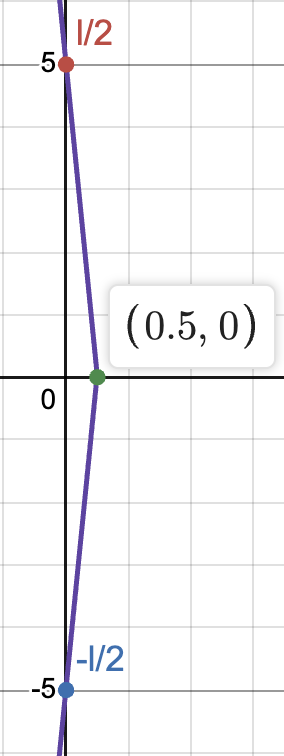
\includegraphics[width=0.2\textwidth]{./image/figure1.png}
                        \caption{Current Distribution of Small Dipole Antenna}
                    \end{figure}
          \end{enumerate}
    \item
          \[l = \frac{\lambda}{2} \text{, } f = 200 \times 10^6 \si{Hz}\text{, } \lambda = 1.5 \si{m} \text{, } R_{in} = R_{rad} = 73 \Omega \text{, }D_0 = 1.64 = 2.15 \si{dB}\]
          \begin{enumerate}[(i)]
              \item $\boxed{l = 0.75}$.
              \item $\boxed{G_0 = 2.51 \si{dB}}$.
              \item We want $P_{rad} = 100 \si{W}$.

                    For a Half-wave Dipole Antenna,
                    \[\frac{1}{2}R_{in} |I_{in}|^2 = P_{rad}\]

                    Therefore,

                    \[|I_{in}| = \sqrt{\frac{2P_{rad}}{R_{in}}} = \boxed{1.66 \si{A}}\]
          \end{enumerate}
\end{enumerate}

\end{document}
